\documentclass[12pt]{article}
\usepackage{amsmath}
\usepackage{amssymb}
\usepackage{geometry}
\usepackage{graphicx}

\geometry{a4paper, margin=1in}

\title{CSE 3504: Project 2}
\author{Isaac Piegat}
\date{12/2/2024}

\begin{document}

\maketitle

\section*{Problem 1:}

\subsection*{1a.}

\begin{center}
    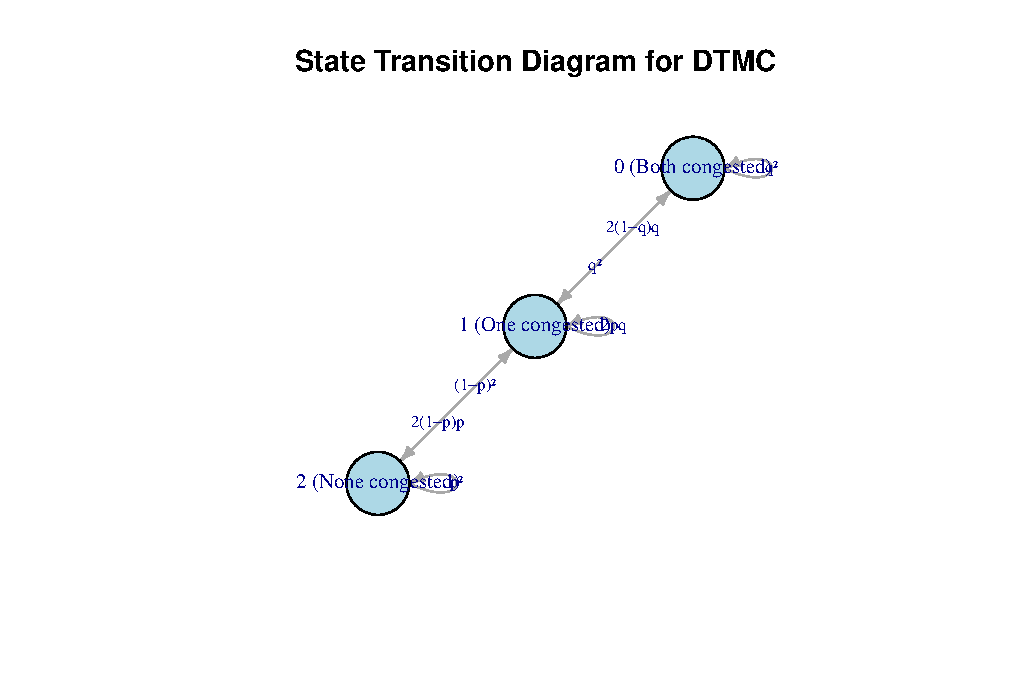
\includegraphics[width=0.8\textwidth]{project2_1a.pdf}
\end{center}

\subsection*{1b.}

\[
P =
\begin{bmatrix}
q^2 & 2(1-q)q & (1-q)^2 \\
q^2 & 2pq & (1-p)^2 \\
p^2 & 2(1-p)p & (1-p)^2
\end{bmatrix}
\]

\subsection*{1c.}

\[
\pi P = \pi, \quad \text{where } \sum_{i} \pi_i = 1
\]

\( p = 0.5 \), \( q = 0.5 \)

\[
P =
\begin{bmatrix}
0.25 & 0.5 & 0.25 \\
0.25 & 0.5 & 0.25 \\
0.25 & 0.5 & 0.25
\end{bmatrix}
\]

R code:

\begin{verbatim}
P <- matrix(c(0.25, 0.5, 0.25,
              0.25, 0.5, 0.25,
              0.25, 0.5, 0.25),
            nrow = 3, byrow = TRUE)

n <- nrow(P)
A <- t(P) - diag(n)  
A[n, ] <- 1         
b <- c(rep(0, n-1), 1)  
steady_state <- solve(A, b)

steady_state
\end{verbatim}

Results:
\[
\pi_0 = 0.25, \quad \pi_1 = 0.5, \quad \pi_2 = 0.25
\]

Thus: \newline
- \( \pi_0 \): Probability that no route is congested is \( 0.25 \). \newline
- \( \pi_1 \): Probability that one route is congested is \( 0.5 \). \newline
- \( \pi_2 \): Probability that both routes are congested is \( 0.25 \).

\subsection*{1d.}

\begin{verbatim}
steady_state_probabilities <- function(p, q) {
  P <- matrix(c(q^2, 2*(1-q)*q, (1-q)^2,
                q^2, 2*p*q, (1-p)^2,
                p^2, 2*(1-p)*p, (1-p)^2),
              nrow = 3, byrow = TRUE)
  n <- nrow(P)
  A <- t(P) - diag(n)  
  A[n, ] <- 1          
  b <- c(rep(0, n-1), 1)  
  steady_state <- solve(A, b)
  return(steady_state)
}

p_values <- seq(0.1, 0.9, by = 0.1)
q <- 0.5
results <- sapply(p_values, function(p) steady_state_probabilities(p, q))

plot(p_values, results[,1], type = "o", col = "blue", ylim = c(0, 1),
     xlab = "Probability p", ylab = "Steady-State Probability",
     main = "Steady-State Probabilities as a Function of p")
lines(p_values, results[,2], type = "o", col = "red")
lines(p_values, results[,3], type = "o", col = "green")
legend("topright", legend = c("No Congestion", "One Congested", "Both Congested"),
       col = c("blue", "red", "green"), lty = 1, pch = 1)
\end{verbatim}

Resulting plot:

\begin{center}
    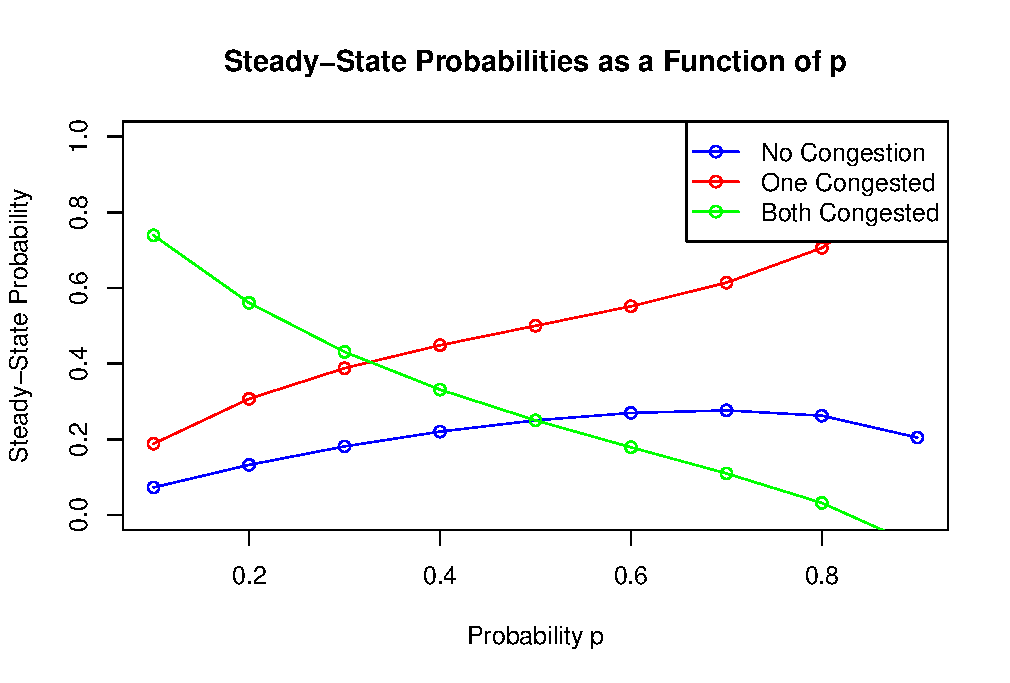
\includegraphics[width=0.8\textwidth]{project2_1d.pdf}
\end{center}

\subsection*{1e.}

\begin{verbatim}
steady_state_probabilities <- function(p, q) {
  P <- matrix(c(q^2, 2*(1-q)*q, (1-q)^2,
                q^2, 2*p*q, (1-p)^2,
                p^2, 2*(1-p)*p, (1-p)^2),
              nrow = 3, byrow = TRUE)
  n <- nrow(P)
  A <- t(P) - diag(n)  
  A[n, ] <- 1          
  b <- c(rep(0, n-1), 1)  
  steady_state <- solve(A, b)
  return(steady_state)
}

q_values <- seq(0.1, 0.9, by = 0.1)
p <- 0.5
results <- sapply(q_values, function(q) steady_state_probabilities(p, q))

plot(q_values, results[,1], type = "o", col = "blue", ylim = c(0, 1),
     xlab = "Probability q", ylab = "Steady-State Probability",
     main = "Steady-State Probabilities as a Function of q")
lines(q_values, results[,2], type = "o", col = "red")
lines(q_values, results[,3], type = "o", col = "green")
legend("topright", legend = c("No Congestion", "One Congested", "Both Congested"),
       col = c("blue", "red", "green"), lty = 1, pch = 1)
\end{verbatim}

Resulting plot:

\begin{center}
    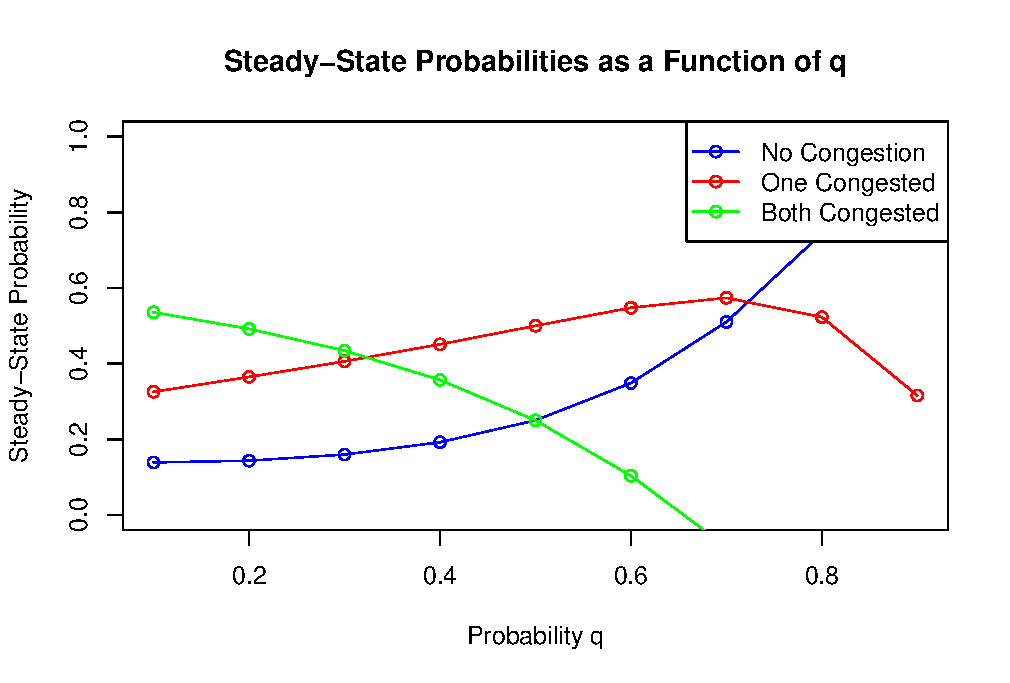
\includegraphics[width=0.8\textwidth]{project2_1e.pdf} % Replace with the path to your plot
\end{center}

\subsection*{1f.}

As $p$ increases, the probability of congestion increases. When it decreases, both one and two congested routes decrease. This means that the higher $p$ there is, there is an overall reduction in congestion. However, as $q$ increases, the probability of both routes being congested increases, while the probabilities of no congestion and one congested route decreases. A higher $q$ then means more ocngested states. 

\section*{Problem 2:}

\subsection*{2a.}

\begin{center}
    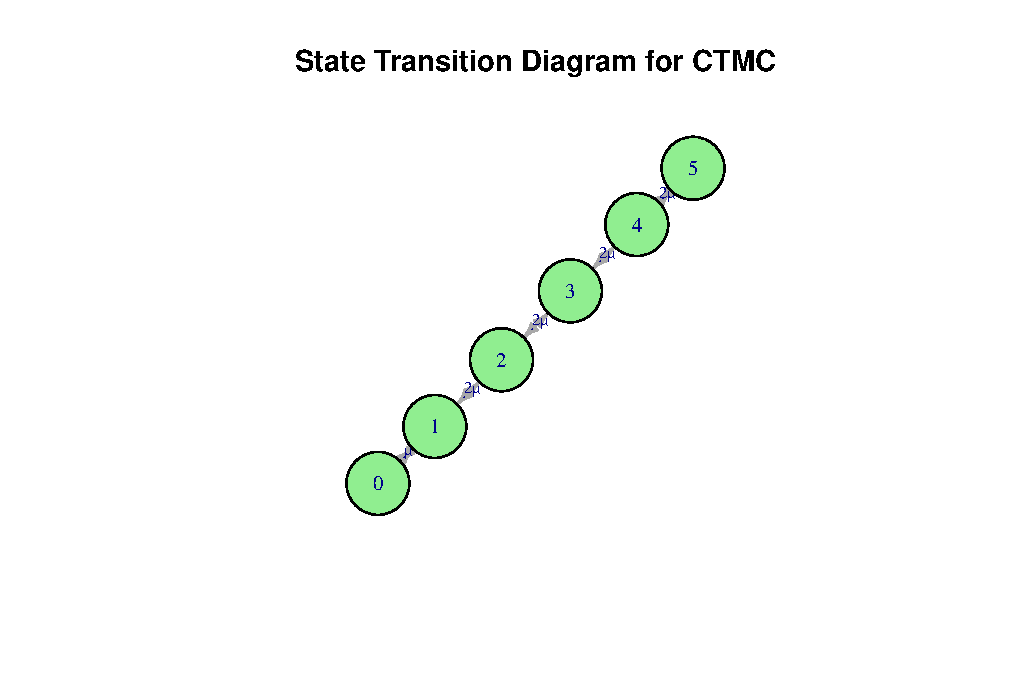
\includegraphics[width=0.8\textwidth]{project2_2a.pdf}
\end{center}

\subsection*{2b.}

\[
Q =
\begin{bmatrix}
-\lambda & \lambda & 0 & 0 & 0 & 0 \\
\mu & -(\lambda + \mu) & \lambda & 0 & 0 & 0 \\
0 & 2\mu & -(\lambda + 2\mu) & \lambda & 0 & 0 \\
0 & 0 & 2\mu & -(\lambda + 2\mu) & \lambda & 0 \\
0 & 0 & 0 & 2\mu & -(\lambda + 2\mu) & \lambda \\
0 & 0 & 0 & 0 & 2\mu & -2\mu
\end{bmatrix}
\]

\subsection*{2c.}

R code:

\begin{verbatim}
lambda <- 6  
mu <- 4      

Q <- matrix(c(
  -lambda, lambda, 0, 0, 0, 0,
  mu, -(lambda + mu), lambda, 0, 0, 0,
  0, 2*mu, -(lambda + 2*mu), lambda, 0, 0,
  0, 0, 2*mu, -(lambda + 2*mu), lambda, 0,
  0, 0, 0, 2*mu, -(lambda + 2*mu), lambda,
  0, 0, 0, 0, 2*mu, -2*mu
), nrow = 6, byrow = TRUE)

n <- nrow(Q)
A <- t(Q)
A[n, ] <- 1  
b <- c(rep(0, n-1), 1)  # Right-hand side
steady_state <- solve(A, b)

p_both_busy <- sum(steady_state[3:6])  
p_turned_away <- steady_state[6]       
\end{verbatim}

The results are:
\[
P(\text{both servers busy}) = 0.55, \quad P(\text{turned away}) = 0.085
\]


\end{document}